\section{Results}
\subsection{Descriptives}
The sex distribution in both cohorts was 49\% male and 51\% female.
Aggression scores slightly declined in boys and girls when they grow up from age 7 to 12 years.
Figure~\ref{fig:meanAggression} shows the mean aggression scores of CBCL and SDQ\@.

\begin{figure}[htpb]
  \centering
  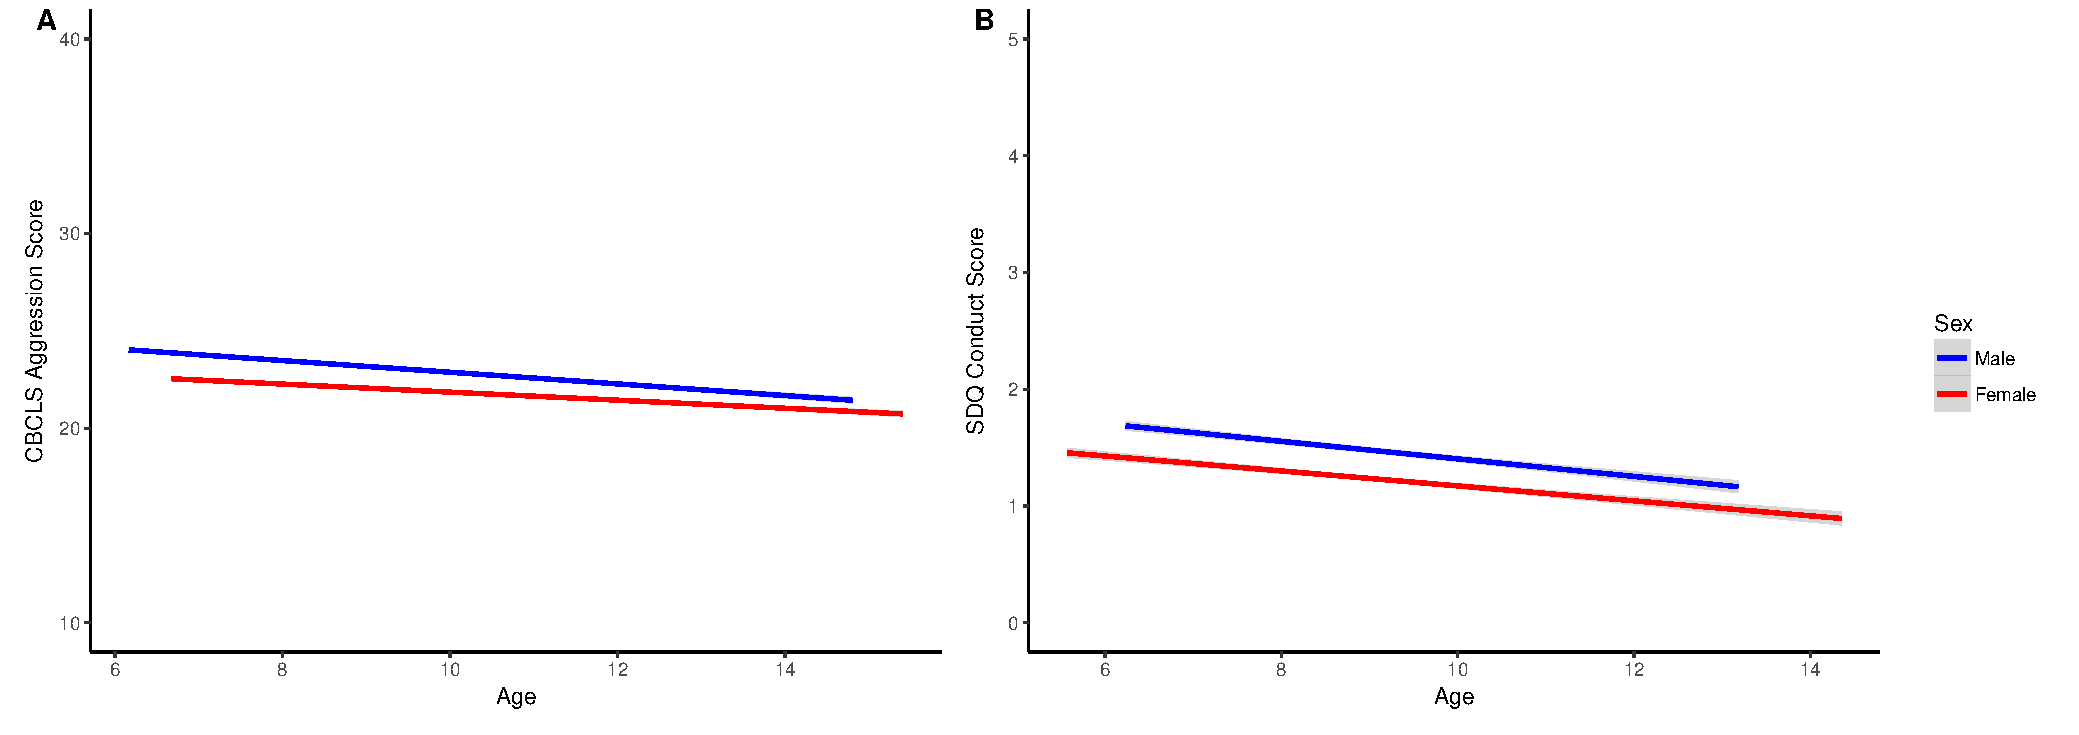
\includegraphics[width=0.99\linewidth]{longHera/figure/aggression_mean_score.pdf}
  \caption[Mean Aggression score]{Mean aggression score for CBCL (Panel A) and SDQ (Panel B) by age and sex.}
  \label{fig:meanAggression}
\end{figure}

Boys scored higher than girls, but for both scales, the sex differences attenuated with age.
Variance is larger for boys than girls for both cohorts at all ages.
Variances in MZ and DZ twins are very similar, ruling out important contributions of sibling interaction or rater contrast effects (Table~\ref{tab:summary})~\cite{Eaves1978, Balakrishnan2014}.

\begin{table}[hbt]
  \centering
  \adjustbox{max width=\columnwidth}{% Table generated by Excel2LaTeX from sheet 'Sheet1'
\begin{tabular}{ccrccrccrcccccc}
  \toprule
  \multicolumn{2}{c}{} &       & \multicolumn{2}{c}{\textbf{Measurement}} &       & \multicolumn{2}{c}{\textbf{Age}} &       & \multicolumn{6}{c}{\textbf{Variance}} \\
  \cmidrule{4-5}\cmidrule{7-8}\cmidrule{10-15}    \textbf{Cohort} & \textbf{n} &       & \textbf{Mean} & \textbf{Sd} &       & \textbf{Median} & \textbf{Range} &       & \textbf{MZM} & \textbf{DZM} & \textbf{MZF} & \textbf{DZF} & \textbf{DOSmf} & \textbf{DOSfm} \\
  \midrule
  \multicolumn{15}{l}{\textbf{NTR}} \\
  7     & 21530 &       & 23.12 & 4.91  &       & 7.35  & 6.17-9.88 &       & 27.83 & 29.2  & 20.15 & 19.09 & 24.28 & 21.85 \\
  10    & 17114 &       & 22.6  & 4.82  &       & 9.96  & 8.71-13.88 &       & 28.71 & 28.82 & 17.56 & 19.4  & 22.58 & 21 \\
  12    & 14352 &       & 21.81 & 4.35  &       & 12.17 & 11.02-15.41 &       & 21.65 & 23.3  & 15.56 & 14.86 & 20.24 & 17.24 \\
  \multicolumn{1}{r}{\textbf{TEDS}} &       &       &       &       &       &       &       &       &       &       &       &       &       &  \\
  7     & 13794 &       & 1.68  & 1.62  &       & 7.04  & 5.57-8.62 &       & 2.86  & 3.08  & 2.15  & 2.39  & 2.63  & 2.65 \\
  9     & 6056  &       & 1.27  & 1.44  &       & 9.01  & 8.08-11.34 &       & 2.46  & 2.38  & 1.75  & 1.8   & 1.76  & 2.29 \\
  12    & 11432 &       & 1.32  & 1.46  &       & 11.44 & 9.79-14.35 &       & 2.19  & 2.48  & 1.78  & 2     & 2.26  & 2.06 \\
  \bottomrule
\end{tabular}%
}
  \caption[Descriptive Summary Statistics of CBCL and SDQ]{Descriptive Summary Statistics}\label{tab:summary}
\end{table}

The longitudinal phenotypic correlations in boys and in girls (see Table~\ref{tab:long_correlation}) are high and reflect strong stability of aggressive behavior between ages 7 and 12.
The twin correlations show a consistent higher correlation within MZ than DZ pairs suggesting additive genetic influences on aggression regardless of assessment instrument (see diagonal in Table~\ref{tab:cross_corr}).
Correlations between same-sex and opposite-sex DZ twin pairs are similar, indicating no qualitative sex-differences.
In addition, twin correlations seem similar across different age groups indicating comparable genetic influences throughout development.
Genetic influences on the covariance of aggression between ages is also to be expected given the higher MZ than DZ cross-twin-cross-age correlations (see off-diagonal estimates in Table~\ref{tab:cross_corr}). 

\begin{table}
  \centering
  % Table generated by Excel2LaTeX from sheet 'Sheet1'
\begin{tabular}{lccr}
  \toprule
  \multicolumn{1}{c}{\textbf{NTR}} & \textbf{7 years} & \textbf{10 years} & \multicolumn{1}{c}{\textbf{12 years}} \\
  \midrule
  7 years &       & 0.70 (0.69, 0.71) & \multicolumn{1}{c}{0.61 (0.59, 0.63)} \\
  10 years & 0.71 (0.7, 0.73) &       & \multicolumn{1}{c}{0.69 (0.67, 0.7)} \\
  12 years & 0.63 (0.61, 0.65) & 0.74 (0.72, 0.75) &  \\
  \midrule
  \multicolumn{1}{c}{\textbf{TEDS}} & \textbf{7 years} & \textbf{9 years} & \multicolumn{1}{c}{\textbf{12 years}} \\
  \midrule
  7 years &       & 0.55 (0.52, 0.58) & \multicolumn{1}{c}{0.5 (0.48, 0.53)} \\
  9 years & 0.58 (0.55, 0.61) &       & \multicolumn{1}{c}{0.55 (0.52, 0.58)} \\
  12 years & 0.55 (0.53, 0.57) & 0.62 (0.59, 0.65) &  \\
  \bottomrule
\end{tabular}%

  \caption[Longitudinal Correlation]{Longitudinal Correlation for NTR and TEDS (Males Below the Diagional and Females Above)}\label{tab:long_correlation}
\end{table}

\begin{landscape}
\begin{table}
  \centering
  \adjustbox{max width=\columnwidth}{% Table generated by Excel2LaTeX from sheet 'Sheet1'
\begin{tabular}{ccccc}
  \toprule
  \textbf{NTR} & \multicolumn{2}{c}{\textbf{7 years}} & \textbf{10 years} & \textbf{12 years} \\
  \midrule
  & \multicolumn{4}{c}{MZ} \\
  7 years & \multicolumn{2}{c}{0.84a (0.82, 0.85) / 0.79b (0.78, 0.81)} & 0.65 (0.63, 0.68) & 0.56 (0.53, 0.59) \\
  10 years & \multicolumn{2}{c}{0.59 (0.57, 0.62)} & 0.83a (0.82, 0.85) / 0.77b (0.75, 0.78) & 0.65 (0.63, 0.67) \\
  12 years & \multicolumn{2}{c}{0.54 (0.51, 0.57)} & 0.56 (0.54, 0.59) & 0.81a (0.79, 0.82) / 0.78b (0.76, 0.79) \\
  \cmidrule{1-5}          & \multicolumn{4}{c}{DZ} \\
  7 years & \multicolumn{2}{c}{0.51a (0.48, 0.54) / 0.44b (0.41, 0.47)} & 0.39 (0.36, 0.42) & 0.34 (0.31, 0.37) \\
  10 years & \multicolumn{2}{c}{0.37 (0.33, 0.4)} & 0.47a (0.44, 0.5) / 0.44b (0.41, 0.47) & 0.35 (0.31, 0.38) \\
  12 years & \multicolumn{2}{c}{0.33 (0.29, 0.37)} & 0.36 (0.32, 0.39) & 0.46a (0.43, 0.49) / 0.47b (0.44, 0.5) \\
  \cmidrule{1-5}          & \multicolumn{4}{c}{DOS} \\
  7 years & \multicolumn{2}{c}{0.44a (0.41, 0.47) / 0.46b (0.43, 0.49)} & 0.32 (0.29, 0.36) & 0.35 (0.31, 0.38) \\
  10 years & \multicolumn{2}{c}{0.32 (0.28, 0.35)} & 0.39a (0.36, 0.42) / 0.44b (0.41, 0.47) & 0.36 (0.33, 0.4) \\
  12 years & \multicolumn{2}{c}{0.29 (0.25, 0.32)} & 0.29 (0.25, 0.32) & 0.53a (0.5, 0.56) / 0.46b (0.43, 0.49) \\
  \midrule
  \textbf{TEDS} & \multicolumn{2}{c}{\textbf{7 years}} & \textbf{9 years} & \textbf{12 years} \\
  \midrule
  &       & \multicolumn{3}{c}{MZ} \\
  7 years & \multicolumn{2}{c}{0.76a (0.74, 0.78) / 0.72b (0.7, 0.74)} & 0.45 (0.41, 0.48) & 0.5 (0.46, 0.53) \\
  9 years & \multicolumn{2}{c}{0.41 (0.37, 0.44)} & 0.8a (0.78, 0.81) / 0.76b (0.74, 0.78) & 0.5 (0.47, 0.53) \\
  12 years & \multicolumn{2}{c}{0.44 (0.41, 0.47)} & 0.48 (0.45, 0.52) & 0.74a (0.72, 0.76) / 0.78b (0.76, 0.8) \\
  \cmidrule{1-5}          & \multicolumn{4}{c}{DZ} \\
  7 years & \multicolumn{2}{c}{0.47a (0.43, 0.5) / 0.44b (0.4, 0.47)} & 0.32 (0.29, 0.36) & 0.32 (0.28, 0.35) \\
  9 years & \multicolumn{2}{c}{0.28 (0.24, 0.32)} & 0.49a (0.45, 0.52) / 0.59b (0.56, 0.62) & 0.29 (0.25, 0.32) \\
  12 years & \multicolumn{2}{c}{0.24 (0.2, 0.28)} & 0.3 (0.26, 0.34) & 0.46a (0.42, 0.49) / 0.52b (0.49, 0.55) \\
  \cmidrule{1-5}          & \multicolumn{4}{c}{DOS} \\
  7 years & \multicolumn{2}{c}{0.46a (0.43, 0.49) / 0.42b (0.39, 0.46)} & 0.2 (0.16, 0.24) & 0.29 (0.25, 0.33) \\
  9 years & \multicolumn{2}{c}{0.23 (0.19, 0.27)} & 0.52a (0.49, 0.55) / 0.45b (0.42, 0.49) & 0.35 (0.31, 0.38) \\
  12 years & \multicolumn{2}{c}{0.26 (0.22, 0.29)} & 0.29 (0.25, 0.33) & 0.52a (0.49, 0.55) / 0.5b (0.47, 0.53) \\
  \bottomrule
\end{tabular}%
}
  \caption[Twin Correlation]{Twin Correlation and Cross Twin Cross Age Correlations}\label{tab:cross_corr}
\end{table}
\end{landscape}

\subsection{Longitudinal Genetic Modelling}
The twin and cross-twin-cross age correlations within NTR and TEDS suggest stable genetic influences on aggression and genetic influences on the stability of aggression.
To investigate the genetic architecture in more detail, a Cholesky decomposition was applied to the raw data in the two studies.
For model comparison I considered the fully saturated genetic model as a reference to test for the significance of common environment (C) shared by twins from the same family, and quantitative sex differences in parameter estimates.
In addition I also investigated a sex specific scalar model, in which I constrained variance components of male and female twins to be proportional to each other, that is I specified equal standardized variance components between the sexes while allowing for differences in unstandardized variances components.
Table~\ref{tab:modelComparison} presents the model fitting results and indicates significant effects for common environmental component in both studies (NTR: $\chi^2_{212}= 127.77$, $p<0.0001$ TEDS: $\chi^2_{212}= 177.28$, $p<0.0001$).
\begin{table}
  \centering
  \adjustbox{max width=\columnwidth}{% Table generated by Excel2LaTeX from sheet 'Sheet1'
\begin{tabular}{ccccccccc}
  \toprule
  \textbf{Reference} & \textbf{Model} & \textbf{Parameters} & \textbf{$-2ll$} & \textbf{df} & \textbf{AIC} & \textbf{$\Delta-2ll$} & \textbf{$\Delta df$} & \textbf{p} \\
  \midrule
  \multicolumn{9}{l}{\textbf{NTR}} \\
  Full Cholesky & Cholesky: Sex moderated AE & 30    & 297589.3 & 55098 & 187393.3 & 127.77 & 12    & $< 0.0001$ \\
  Full Cholesky & Cholesky: no-sex moderated ACE & 24    & 298058.36 & 55104 & 187850.36 & 596.83 & 18    & $< 0.0001$ \\
  Full Cholesky & Cholesky: scaled sex ACE & 27    & 297563.15 & 55101 & 187361.15 & 101.63 & 15    & $< 0.0001$ \\
  \multicolumn{9}{l}{\textbf{TEDS}} \\
  Full Cholesky & Cholesky: Sex moderated AE & 30    & 101529.26 & 30983 & 39563.26 & 177.29 & 12    & $< 0.0001$ \\
  Full Cholesky & Cholesky: no-sex moderated ACE & 24    & 101545.1 & 30989 & 39567.1 & 193.13 & 18    & $< 0.0001$ \\
  Full Cholesky & Cholesky: scaled sex ACE & 27    & 101397.13 & 30986 & 39425.13 & 45.16 & 15    & $< 0.0001$ \\
  \multicolumn{9}{l}{\textbf{Combined}} \\
  \textbf{Cholesky: Study specific parameters} &       & \textbf{84} & \textbf{398813.5} & \textbf{86057} & \textbf{226699.5} &       &       &  \\
  Cholesky: Study specific parameters & Cholesky: Combined estimates & 54    & 399248.6 & 86087 & 227074.6 & 435.073 & 30    & $< 0.0001$ \\
  \cmidrule{1-8}    
\end{tabular}%
}
  \caption[Model Comparison of Longitudinal Analysis]{Model Comparison of Longitudinal Analysis.
  The final model is indicated in bold.}\label{tab:modelComparison}
\end{table}
Constraining parameters to be the same for boys and girls (NTR: $\chi^2_{218}= 596.82$, $p<0.0001$; TEDS: $\chi^2_{218}= 193.12$, $p<0.0001$), as well as constraining male variance components proportional to female estimates (NTR: $\chi^2_{215}= 101.63$, $p<0.0001$; TEDS: $\chi^2_{215}= 45.15$, $p<0.0001$) resulted in a significant worsening of model fit, which suggests small but significant sex differences.
In order to test for similarities in genetic architecture of aggression as assessed with the CBCL and the SDQ I tested for equal standardized components by constraining parameters of TEDS to be proportional of those in NTR\@.
This resulted in a significant worse fit compared to study specific estimates ($\chi^2_{230}= 435.07$, $p<0.0001$).
Thus, there are significant differences between the genetic architecture of aggression based on the CBCL (NTR) and the SDQ (TEDS).
The differences are small, as may be seen from the study specific variance and covariance components for NTR and TEDS in Table~\ref{tab:var_components}.
%\begin{landscape}
\begin{table}
  \centering
  \adjustbox{max width=\columnwidth}{% Table generated by Excel2LaTeX from sheet 'Sheet1'
\begin{tabular}{llll}
  \toprule
      & \multicolumn{3}{c}{\textbf{A}} \\
\cmidrule{2-4} \textbf{NTR} & \textbf{7 years} & \textbf{10 years} & \textbf{12 years} \\
\midrule
7 years & 19.4 (17.85, 21.1) / 15.39 (14.36, 16.23) & 15.03 (13.76, 16.34) & 13.76 (12.63, 14.87) \\
10 years & 11.14 (10.26, 11.87) & 19.72 (18.21, 21.33) / 14.05 (13.03, 14.91) & 15.24 (14.05, 16.43) \\
12 years & 9.25 (8.44, 9.95) & 9.71 (8.85, 10.48) & 16.41 (15.02, 17.75) / 9.64 (8.65, 10.65) \\
      &       &       &  \\
7 years & 0.66 (0.6, 0.71) / 0.78 (0.74, 0.8) & 0.72 (0.65, 0.79) & 0.82 (0.75, 0.9) \\
10 years & 0.83 (0.78, 0.86) & 0.68 (0.63, 0.74) / 0.76 (0.72, 0.78) & 0.79 (0.72, 0.85) \\
12 years & 0.87 (0.81, 0.9) & 0.83 (0.77, 0.9) & 0.69 (0.63, 0.74) / 0.62 (0.56, 0.68) \\
      &       &       &  \\
\cmidrule{2-4}\textbf{TEDS} & \textbf{7 years} & \textbf{9 years} & \textbf{12 years} \\
      \midrule
7 years & 1.88 (1.64, 2.16) / 1.44 (1.22, 1.63) & 1.06 (0.83, 1.37) & 1.1 (0.94, 1.28) \\
9 years & 0.71 (0.57, 0.86) & 1.45 (1.18, 1.74) / 0.78 (0.63, 0.94) & 0.98 (0.81, 1.19) \\
12 years & 0.83 (0.7, 0.96) & 0.71 (0.58, 0.85) & 1.4 (1.21, 1.6) / 1.08 (0.94, 1.23) \\
      &       &       &  \\
7 years & 0.62 (0.55, 0.71) / 0.63 (0.53, 0.7) & 0.67 (0.51, 0.87) & 0.74 (0.62, 0.85) \\
9 years & 0.63 (0.5, 0.76) & 0.59 (0.47, 0.69) / 0.42 (0.34, 0.52) & 0.64 (0.53, 0.77) \\
12 years & 0.78 (0.66, 0.89) & 0.68 (0.55, 0.81) & 0.57 (0.5, 0.65) / 0.55 (0.48, 0.63) \\
      &       &       &  \\
      \midrule
      & \multicolumn{3}{c}{\textbf{C}} \\
\cmidrule{2-4} \textbf{NTR} & \textbf{7 years} & \textbf{10 years} & \textbf{12 years} \\
      \midrule
7 years & 5.48 (3.76, 7.14) / 0.22 (0, 0.93) & 4.01 (2.53, 5.45) & 1.87 (0.72, 3.12) \\
10 years & 0.17 (-0.01, 0.76) & 4.47 (2.73, 6.2) / 0.18 (0, 0.84) & 2.27 (1.06, 3.59) \\
12 years & 0.28 (0, 0.85) & 0.34 (-0.38, 0.99) & 3.1 (1.94, 4.47) / 2.42 (1.59, 3.28) \\
      &       &       &  \\
7 years & 0.19 (0.13, 0.24) / 0.01 (0, 0.05) & 0.19 (0.12, 0.25) & 0.11 (0.04, 0.18) \\
10 years & 0.01 (0, 0.06) & 0.15 (0.1, 0.21) / 0.01 (0, 0.04) & 0.12 (0.06, 0.18) \\
12 years & 0.03 (0, 0.08) & 0.03 (-0.03, 0.08) & 0.13 (0.08, 0.18) / 0.16 (0.1, 0.21) \\
      &       &       &  \\
\cmidrule{2-4} \textbf{TEDS} & \textbf{7 years} & \textbf{9 years} & \textbf{12 years} \\
      \midrule
7 years & 0.44 (0.18, 0.67) / 0.24 (0.09, 0.45) & 0.3 (0.03, 0.56) & 0.24 (0.09, 0.41) \\
9 years & 0.21 (0.08, 0.37) & 0.49 (0.25, 0.79) / 0.65 (0.48, 0.83) & 0.32 (0.14, 0.48) \\
12 years & 0.16 (0.06, 0.29) & 0.21 (0.08, 0.35) & 0.47 (0.3, 0.65) / 0.47 (0.34, 0.62) \\
      &       &       &  \\
7 years & 0.14 (0.06, 0.22) / 0.1 (0.04, 0.19) & 0.19 (0.02, 0.34) & 0.16 (0.06, 0.26) \\
9 years & 0.19 (0.07, 0.32) & 0.2 (0.1, 0.31) / 0.36 (0.27, 0.44) & 0.21 (0.09, 0.31) \\
12 years & 0.15 (0.05, 0.26) & 0.21 (0.08, 0.32) & 0.19 (0.12, 0.26) / 0.24 (0.17, 0.31) \\
      &       &       &  \\
      \midrule
      & \multicolumn{3}{c}{\textbf{E}} \\
\cmidrule{2-4} \textbf{NTR} & \textbf{7 years} & \textbf{10 years} & \textbf{12 years} \\
      \midrule
7 years & 4.67 (4.38, 4.99) / 4.13 (3.89, 4.38) & 1.89 (1.6, 2.18) & 1.05 (0.75, 1.36) \\
10 years & 2.1 (1.88, 2.34) & 4.79 (4.47, 5.15) / 4.32 (4.04, 4.63) & 1.86 (1.57, 2.16) \\
12 years & 1.16 (0.96, 1.38) & 1.65 (1.42, 1.89) & 4.31 (3.98, 4.67) / 3.51 (3.26, 3.78) \\
      &       &       &  \\
7 years & 0.16 (0.15, 0.17) / 0.21 (0.2, 0.22) & 0.09 (0.08, 0.1) & 0.06 (0.05, 0.08) \\
10 years & 0.16 (0.14, 0.18) & 0.17 (0.15, 0.18) / 0.23 (0.22, 0.25) & 0.1 (0.08, 0.11) \\
12 years & 0.11 (0.09, 0.13) & 0.14 (0.12, 0.16) & 0.18 (0.17, 0.2) / 0.23 (0.21, 0.24) \\
      &       &       &  \\
\cmidrule{2-4} \textbf{TEDS} & \textbf{7 years} & \textbf{9 years} & \textbf{12 years} \\
      \midrule
7 years & 0.69 (0.64, 0.75) / 0.61 (0.56, 0.66) & 0.21 (0.14, 0.27) & 0.15 (0.11, 0.2) \\
9 years & 0.2 (0.16, 0.23) & 0.53 (0.47, 0.6) / 0.4 (0.36, 0.45) & 0.23 (0.18, 0.29) \\
12 years & 0.07 (0.04, 0.11) & 0.13 (0.09, 0.16) & 0.58 (0.53, 0.64) / 0.4 (0.37, 0.43) \\
      &       &       &  \\
7 years & 0.23 (0.21, 0.25) / 0.27 (0.24, 0.29) & 0.13 (0.09, 0.17) & 0.1 (0.07, 0.13) \\
9 years & 0.17 (0.14, 0.21) & 0.21 (0.19, 0.25) / 0.22 (0.2, 0.25) & 0.15 (0.12, 0.19) \\
12 years & 0.07 (0.04, 0.1) & 0.12 (0.09, 0.15) & 0.24 (0.22, 0.26) / 0.2 (0.19, 0.22) \\
  \bottomrule
\end{tabular}%
}
  \caption[Unstandardized and Standardized Variance and Covariance Component]{Unstandardized and Standardized Variance and Covariance Component (Diagional,
    First Number is for Male, Second is for Female.
    Diagonals, Above is Male, Below is Female)}\label{tab:var_components}
\end{table}
%\end{landscape}
The heritability of aggression at ages 7, 9/10 and 12 year ranges between 42\% and 78\%.  The lowest estimate (42\%) is observed for females at age 10 in the TEDS sample, while the highest estimates are observed for females at age 7 (78\%) and age 10 (76\%) in the NTR sample.
A number of differences could be observed between NTR and TEDS.
Heritability is somewhat lower in TEDS than NTR across sexes and differences between boy and girl estimates are slightly larger in NTR.
Nevertheless, overall both studies are rather similar with respect to the influence of genetic and environmental components on aggressive behavior, despite the differences in assessment instruments.
Partitioning of genetic effects into influences from prior ages demonstrated that the latent genetic factor in T1 is a major contributor to the genetic variance at T2 and T3, indicating that preexisting genetic factors play an increasingly important role in explaining variation in aggressive behavior (see Table~\ref{tab:hera}).
The influence of T1 on subsequent ages is stronger in NTR than TEDS, which is also reflected by the relatively larger longitudinal correlation in NTR.
This stability in underlying genetic effects is also reflected in the high genetic correlations (Table~\ref{tab:genetic_correlation}).
Genetic correlations are in the ranges of .76-.85 for NTR and .64 and .77 for TEDS.
These high genetic correlation in combination with the significant genetic influences on the stability of aggressive behavior indicates that genes are the major driving force of the persistence of aggressive behavior throughout childhood regardless of the assessment instrument. 

\begin{table}
  \centering
  \adjustbox{max width=\columnwidth}{% Table generated by Excel2LaTeX from sheet 'Sheet1'
\begin{tabular}{llll}
\hline
      & \multicolumn{3}{c}{\textbf{Male}} \\
\cline{2-4}\multicolumn{1}{c}{\textbf{Cohort}} & \multicolumn{1}{c}{\textbf{A}} & \multicolumn{1}{c}{\textbf{C}} & \multicolumn{1}{c}{\textbf{E}} \\
\hline
\multicolumn{4}{l}{\textbf{NTR}} \\
7 years & 0.66 (0.6, 0.71)  & 0.19 (0.13, 0.24)  & 0.16 (0.15, 0.17)  \\
10 years & 0.68 (0.63, 0.74)     [0.4, 0.28] & 0.15 (0.1, 0.21) [0.1, 0.05] & 0.17 (0.15, 0.18) [0.03, 0.14] \\
12 years & 0.69 (0.63, 0.74) [0.41, 0.11, 0.17] & 0.13 (0.08, 0.18) [0.03, 0.02, 0.08] & 0.18 (0.17, 0.2) [ 0.01, 0.02, 0.15] \\
\multicolumn{4}{l}{\textbf{TEDS}} \\
7 years & 0.62 (0.55, 0.71)  & 0.14 (0.06, 0.22) & 0.23 (0.21, 0.25) \\
9 years & 0.59 (0.47, 0.69) [0.24, 0.35] & 0.2 (0.1, 0.31) [0.08, 0.12] & 0.21 (0.19, 0.25) [0.02, 0.19 ] \\
12 years & 0.57 (0.5, 0.65) [0.26, 0.07, 0.24] & 0.19 (0.12, 0.26) [0.06, 0.03, 0.1] & 0.24 (0.22, 0.26) [0.01, 0.04 , 0.19] \\
\hline
& \multicolumn{3}{c}{\textbf{Female}} \\
\hline
\multicolumn{4}{l}{\textbf{NTR}} \\
\hline
7 years & 0.78 (0.74, 0.8)  & 0.01 (0, 0.05)  & 0.21 (0.2, 0.22)  \\
10 years & 0.76 (0.72, 0.78) [0.43, 0.33] & 0.01 (0, 0.04) [0.01, 0] & 0.23 (0.22, 0.25) [0.06, 0.17] \\
12 years & 0.62 (0.56, 0.68) [0.36, 0.1, 0.16] & 0.16 (0.1, 0.21) [0.02, 0.02, 0.12] & 0.23 (0.21, 0.24) [0.03, 0.02, 0.18] \\
\multicolumn{4}{l}{\textbf{TEDS}} \\
7 years & 0.63 (0.53, 0.7) & 0.1 (0.04, 0.19) & 0.27 (0.24, 0.29) \\
9 years & 0.42 (0.34, 0.52) [0.19, 0.23 ] & 0.36 (0.27, 0.44) [0.1, 0.25] & 0.22 (0.2, 0.25) [0.03, 0.17] \\
12 years & 0.55 (0.48, 0.63) [0.25, 0.1, 0.2] & 0.24 (0.17, 0.31) [0.05, 0.01, 0.18] & 0.2 (0.19, 0.22)  [0, 0.02, 0.18] \\
\hline
\end{tabular}

}
  \caption[Partioned Variance Components]{Variance component are partitioned into effects due to effects from different time points (brackets).
    The first, second and third number are effects due to first, second or third genetic/environmental factors, respectively.
    Confidence intervals (95\%) for the standardized variance component are given in parentheses.
}\label{tab:hera}
\end{table}

\begin{table}
  \centering
  \adjustbox{max width=\columnwidth}{\begin{tabular}{lccr}
  \toprule
  \multicolumn{1}{c}{\textbf{NTR}} & \textbf{7 years} & \textbf{10 years} & \multicolumn{1}{c}{\textbf{12 years}} \\
  \midrule
  7 years &       & 0.76 (0.73, 0.78) & \multicolumn{1}{c}{0.76 (0.72, 0.8)} \\
  10 years & 0.77 (0.72, 0.8) &       & \multicolumn{1}{c}{0.83 (0.79, 0.88)} \\
  12 years & 0.77 (0.73, 0.81) & 0.85 (0.81, 0.89) &  \\
  \midrule
  \multicolumn{1}{c}{\textbf{TEDS}} & \textbf{7 years} & \textbf{9 years} & \multicolumn{1}{c}{\textbf{12 years}} \\
  \midrule
  7  years &       & 0.67 (0.57, 0.76) & \multicolumn{1}{c}{0.67 (0.58, 0.75)} \\
  9  years & 0.64 (0.54, 0.76) &       & \multicolumn{1}{c}{0.77 (0.68, 0.85)} \\
  12 years & 0.68 (0.6, 0.76) & 0.69 (0.61, 0.78) &  \\
  \bottomrule
\end{tabular}%
}
  \caption[Genetic Twin Correlations]{Upper triangle displays female and lower male genetic correlation.
    The 95\% confidence intervals are given in parentheses.
}\label{tab:genetic_correlation}
\end{table}
